\documentclass{ucetd}
\usepackage{subfigure,epsfig,amsfonts}
\usepackage[sort&compress,numbers]{natbib}
\usepackage{amsmath}
\usepackage{amssymb}
\usepackage{amsthm}
\usepackage{braket}
\usepackage{mathrsfs}
% \usepackage{cancel}

% Following 2 lines silence the \underline warnings.
\usepackage{silence}
\WarningFilter{latex}{Command}

\usepackage{sectsty}
\usepackage{float}
\usepackage{graphicx}
\usepackage{color,soul}
% \usepackage[colorinlistoftodos]{todonotes}
\usepackage{lipsum}

% \usepackage{tikz}
% \usepackage{circuitikz}
% \usepackage{tikz-timing}
% \usetikzlibrary{arrows.meta,decorations.pathmorphing,decorations.pathreplacing,positioning,shapes,fadings}

%Modify directory for loading graphics
\graphicspath{{figures/}}
%Extra
% \usepackage{filecontents}
\usepackage{bm}
\usepackage{braket}
\usepackage{setspace}
\usepackage{listings}
\usepackage{multicol}
\usepackage{verbatim}
\usepackage{physics}
\usepackage{dsfont}
\usepackage{pdflscape}
\usepackage{adjustbox}
\usepackage{blkarray}
\usepackage{colortbl}
\usepackage{hyperref}
% \usepackage{adjustbox}
% \usepackage{cancel}
\usepackage{rotating}

\renewcommand{\bibname}{References}





%% Use these commands to set biographic information for the title page:
\title{your thesis title here}
\author{your name here}
\department{Pritzker School of Molecular Engineering}
\division{Pritzker School of Molecular Engineering}
\degree{Doctor of Philosophy}
\date{Month and Year of Graduation}  % date of degree awarding, not the date of the defense

%% Use these commands to set a dedication and epigraph text
\dedication{Dedication text}
%\epigraph{Epigraph Text}

\usepackage{caption}
%\captionsetup{font=footnotesize}
\usepackage{pdfpages}

\begin{document}



\maketitle

\makecopyright
\makededication
%\makeepigraph

%% Make the various tables of contents
\tableofcontents
\cleardoublepage
\phantomsection
\listoffigures
\cleardoublepage
\phantomsection
\listoftables
\newpage

\begin{center}
    \textit{This thesis represents the motivations, results, and conclusions from the following works}:
    \\
    \begin{enumerate}

        \item[] 
    \end{enumerate}

\end{center}
\newpage
 
\acknowledgments
\begin{center}
    \textit{XYZ...}
\end{center}

XYZ

\abstract
Abstract


\mainmatter

% Chapter 1

\chapter{Introduction} % Main chapter title

\label{ch:intro} % For referencing the chapter elsewhere, use \ref{Chapter1} 

%----------------------------------------------------------------------------------------

% Define some commands to keep the formatting separated from the content 
\newcommand{\keyword}[1]{\textbf{#1}}
\newcommand{\tabhead}[1]{\textbf{#1}}
\newcommand{\code}[1]{\texttt{#1}}
\newcommand{\file}[1]{\texttt{\bfseries#1}}
\newcommand{\option}[1]{\texttt{\itshape#1}}
% \newcommand{\enquote}[1]{``#1"}
%----------------------------------------------------------------------------------------

In 1965 at Bell Labs, Arno Penzias and Robert Wilson serendipitously detected ``noise" with their microwave antenna.  This noise was isotropic (same in all directions) and homogenous (same in all locations), and was ultimately the measurement of the Cosmic Microwave Background; radiation from the early universe.
\begin{equation}
    I(\nu,T) = \frac{2h\nu^2}{c^2}\frac{1}{e^{\frac{h\nu}{k_B T}} -1}
    \label{eq:blackbody}
\end{equation}
The temperature spectrum of the Cosmic Microwave Background (CMB) was measured to be a near-perfect black-body (Eq.~\ref{eq:blackbody}), with a mean temperature of~\cite{burke_graham-smith_wilkinson_2019}:
\begin{equation}
    T_{\text{CMB}} = 2.725\,K
\end{equation}
The spectrum lies in the infra-red range of the electromagnetic spectrum, and peaks at a wavelength $\lambda = 1.5\,\text{mm}$ (Figure~\ref{fig:cobe_power_spectra}). 

This near-perfect black-body is understood to originate during the early universe by the rapid collision of photons with free electrons (Thompson scattering), to keep radiation in thermal equilibrium with hot dense matter.  As the universe expanded and cooled, however, this spectrum kept its same form~\cite{weinberg_cosmo}.  Because it formed during the early universe, the CMB is a backlight into not only early universe properties, but also late universe physics such as large-scale structure and dark matter.  The CMB, therefore, carries a wealth of information about the fundamental physics of our universe.

\begin{figure}[t]
    \centering
    \includegraphics[width = \textwidth]{Figures/cobe_power_spec.pdf}
    \caption{Left: Spectrum of the CMB from the COBE satellite~\cite{1994ApJ...420..439M}.  The deviation from an ideal blackbody is magnified $\times\,400$ in the bottom panel.  Right: First-year maps from the COBE Differential Microwave Radiometer in 1992~\cite{1992ApJ...396L...1S}.}
    \label{fig:cobe_power_spectra}
\end{figure}

\section{The Expanding Universe}
The evolution of the universe can be described using an extension of Einstein's equations.  To measure distances in an expanding universe, we employ the metric $ds$, which depends on the curvature of the space, with curvature $\kappa$:
\begin{equation}
    ds^2 = -c^2dt^2 + a(t)^2[dr^2 + S_\kappa (r^2)d\Omega^2]\text{ ,}
\end{equation}
where
\begin{equation}
    d\Omega^2\equiv d\theta^2 + \sin^2\theta d\phi^2
\end{equation}
and
\begin{equation}
    S_\kappa(r) = \begin{cases} R\sin(r/R) & (\kappa = +1) \\
  r & (\kappa = 0) \\
   R\sinh(r/R) & (\kappa = -1)\end{cases}
\end{equation}
Here, we consider the scale of the universe as a function of time $a(t)$, which relates to the redshift $z$ as
\begin{equation}
    a(t) = \frac{1}{a+z}\text{ ,}
\end{equation}
where we set today's $a=1$.  If $a(t)$ is increasing, then the object is ``red-shifted", or a decrease in frequency.  This relationship can be expanded for nearby sources:
\begin{equation}
    a(t)\approx a(t_0)[1+(t-t_0)H_0+ \ldots ]
\end{equation}
where we've introduced the Hubble Constant $H_0$.  The Hubble Constant quantifies the expansion of our universe:
\begin{equation}
    H_0\equiv \bigg(\frac{\dot{a}}{a}\bigg )_{t=t_0}\; .
\end{equation}
In recent decades, astronomers and cosmologists have worked to determine the exact value of $H_0$ using both early- and late-universe physics.  As the two methods return differing values of the Hubble Constant, this field continues to evolve with new statistical methods and precision instrumentation.

\section{The Three Equations of the Universe}
The dynamics of the universe are neatly described by three equations, which connect its curvature to the energy density $\rho$ and pressure $P$.

\noindent
\textbf{Friedmann Equation}:  Stemming from Einstein's relativistic field equations, the Friedmann equation describes a homogenous and isotropic universe:  
\begin{equation}
    \bigg ( \frac{\Dot{a}}{a} \bigg ) = \frac{8\pi G}{3c^2}\rho(t) - \frac{\kappa c^2}{R_0}\frac{1}{a(t)}
\end{equation}
where $\rho$ is the energy density, $G$ is the gravitational constant, $c$ is the speed of light, $\kappa$ is the curvature parameter, and $R_0$ is the radius of curvature at present time $t=0$.  The energy density is evolving, and made up of matter ($\rho_m=\rho_{m0}a^{-3}$), radiation ($\rho_r=\rho_{r0}a^{-4}$), and a cosmological constant ($\rho_{\Lambda}=\rho_{\Lambda 0}$), thus the Friedman equation takes the form:
\begin{equation}
    \frac{H^2}{H_0^2} = \frac{\Omega_{r0}}{a^4} + \frac{\Omega_{m0}}{a^3} + \Omega_{\Lambda 0} + \frac{1-\Omega_0}{a^2}
\end{equation}
where we normalize the energy density $\rho$ by the critical density $\rho_c(t)$, where $\rho_c(t) = \frac{3c^2}{8\pi G}$~\cite{ryden_2016}.  This results in the new variable:
\begin{equation}
    \Omega(t) = \frac{\rho(t)}{\rho_c(t)}
\end{equation}
Today, cosmologists assume a standard model of cosmology, which is referred to as the ``$\Lambda$CDM model".  The $\Lambda$CDM model assumes a flat $\Omega(t)=1$ universe, consisted mostly of baryonic ($\Omega_b h^2$) and cold dark matter ($\Omega_c h^2$) densities.  We will discuss this model further in the next sections.

\noindent
\textbf{Fluid Equation}:  Energy conservation can also be applied to describe the dynamics of the universe through the first law of thermodynamics (Eq.~\ref{eq:thermo1}).  This implies the sum of gravitational potential and kinetic energy of expansion is conserved~\cite{ryden_2016}.
\begin{equation}
    dQ = dE + PdV
    \label{eq:thermo1}
\end{equation}
\begin{equation}
    \dot{\rho} + \frac{3\dot{a}}{a}(\rho + P) = 0
    \label{eq:fluid_universe}
\end{equation}
\noindent
Solving the fluid equation (with $P=w\rho$) yields the equation of state:
\begin{equation}
    \rho \propto a^{-3(1+w)}
\end{equation}
with the time-independent $w$~\cite{weinberg_cosmo}.  For example, in the case of a cold matter dominated universe (e.g. dust, $P = 0$) $\rho\propto a^{-3}$, and in a hot matter universe (e.g. radiation, $P=\rho/3$) $\rho\propto a^{-4}$.

\noindent
\textbf{Acceleration Equation}: Combining the first two equations, which constrain an energy conserved universe, yields the acceleration equation describing how our universe expands over time.  
\begin{equation}
    \frac{\ddot{a}}{a} = - \frac{4\pi G}{3 c^2} (\rho + 3 P)
\end{equation}
\begin{figure}
    \centering
    \includegraphics[width=\textwidth]{Figures/universe.pdf}
    \caption{The history of the universe as we understand it today.  After the Big Bang, the CMB is emitted during the Recombination era at around 380,000.  The photons emitted then traversed large-scale structure to get to our detectors, and therefore we can study late universe large-scale structure through measurements of the CMB.  Credit: ESA/Planck Team~\cite{NASApic}, re-touched by Chesmore.}
    \label{fig:universe_timeline}
\end{figure}
\section{The Case for Cosmic Inflation}
Three pillars provide evidence for the Big Bang Theory, whereupon our universe came into existence.

\noindent
\textbf{The Expanding Universe}: As we've previously discussed in this chapter, the universe is predicted to be currently expanding.  This has been studied and proven by observations of late-universe objects like galaxies~\cite{1999ApJ...517..565P}.  By measuring the velocity and distance of an object, scientists determined (using the Hubble Law) objects in the past were closer together, and today are farther apart.  

\noindent
\textbf{The Cosmic Microwave Background}:
Radiation from a source of known temperature is described by a black-body spectrum.  We've introduced the CMB as radiation from the early universe.  We've also introduced the CMB as a blackbody spectrum.  It can be shown that, in an expanding universe, the blackbody will maintain its shape, its temperature will decrease as the wavelength shifts lower.  Therefore, the CMB serves as evidence of a dense hot radiation source before the universe expanded, with a consistent black-body shape.

\noindent
\textbf{Abundance of Light Elements}:  Such an abundance of light elements in today's universe suggests a hot, dense beginning to the universe.  As the universe cooled and expanded, light particles formed by a fusion process called Big Bang Nucleosynthesis (BBN).  The amount of light particles measured today are in agreement with predictions made by BBN.

These three pillars indicate a valid understanding of cosmology, but this cosmology remains incomplete.  Problems which remain are listed below.  The theory of inflation has the potential to explain the mentioned puzzles.

\begin{enumerate}
    \item Flatness problem:  Measurements of the observable universe present a nearly flat spatial geometry ($\Omega_{\text{total}}=1$).  This would imply a flat geometry at the initial moments of our universe as well.  But for what reason would the universe begin with a flat geometry?  Inflation answers this by suggesting our universe might have curvature, but this rapid expansion blows up any curvature such that the tiny amount we can observe appears flat. 
    \item Horizon problem:  The sky appears remarkably (and statistically) uniform in all directions.  The CMB confirms this, as we measure this radiation to be uniform to one part in $100,000$.  The particle horizon distance is only $2^{\circ}$, so how could the entire sky be so nearly uniform?  Inflation solves this because such an accelerated expansion creates a paradigm where all the observed sky has a chance to come into causal contact.
    \item Magnetic monopole problem:  Magnetic monopoles are analogous to electrons, which would emit a magnetic charge.  However, we have never measured a single monopole in our universe, nor do we know that they exist.  Meanwhile, the Grand Unified Theory (GUT) predicts an extremely low density of magnetic monopoles; GUT predicts one monopole per Hubble radius.  Inflation solves this by diluting the expected number of monopoles thus explaining why we have not measured a single one.
\end{enumerate}
\section{$\Lambda$CDM Cosmology}
Today, the universe is described by the $\Lambda$CDM model, which assumes a flat universe ($\Omega_{\text{tot}}=1$) which is expanding at an accelerating rate, and is dominated by cold dark energy and cold dark matter.  Further, the $\Lambda$CDM model assumes dark energy taking the form of a cosmological constant $\Lambda$, which is expressed as a constant energy density:
\begin{equation}
    \rho_\Lambda = \frac{c^2}{8\pi G}\Lambda 
\end{equation}
The $\Lambda$CDM model neatly models the universe in six parameters: the baryonic density $\Omega_b\,h^2$, the cold dark matter density $\Omega_c\,h^2$, $\ln(10^{10}A_s)$, the spectral index of inflation $n_s$, the size of the acoustic horizon at decoupling 100\,$\theta_{*}$, and the reionization optical depth $\tau$.  Further, the standard model assumes a constant number of neutrino $N_{\text{eff}}$ and sum of neutrino masses $\Sigma m_\nu$. The most up-to-date values are listed in Table~\ref{tab:cosmology_recent_results}.  All of these parameters impact the shape of the CMB spectra which we measure today.

\section{The CMB Temperature Power Spectra}
The Cosmic Microwave Background carries rich science in its temperature and polarization spectra.  The CMB temperature spectrum can be decomposed into spherical harmonics, which result in power spectra as a function of multipole moment $\ell$, where $\ell\approx180/\theta$ and $\theta$ is angular scale on the sky.  The temperature fluctuations of the CMB are decomposed into spherical harmonics:
\begin{equation}
\frac{\delta T}{T}(\theta,\phi) = \sum_{\ell=2}^{\infty} \sum_{m=-\ell}^{\ell} a_{\ell m} Y_{\ell m}(\theta,\phi)
    \label{eq:cmb_temp}
\end{equation}

where $\ell$ and $m$ are multipoles of the spherical harmonic $Y_{\ell m}$, $a_{\ell m}$ are expansion coefficients, and $\theta$ and $\phi$ represent the angular position on the sky.  You'll notice the first summation of Equation~\ref{eq:cmb_temp} begins at $\ell=2$ rather than $\ell=0$; the $\ell=1$ coefficient corresponds to the earth's motion with respect to the CMB, and the $\ell=0$ coefficient is the mean temperature of the CMB, so we neglect those terms.  The coefficients $a_{\ell m}$ are independent variables, and relate to the CMB's angular power spectra via:
\begin{equation}
    C_\ell^{TT} = \frac{1}{2\ell +1} \sum_{m=-\ell}^{m=\ell} |a_{\ell m}|^2
\end{equation}

This is the temperature power spectrum of the CMB.  Figure~\ref{fig:measured_cmb_spec} shows the measured CMB temperature power spectrum from the Atacama Cosmology Telescope, the South Pole Telescope, and WMAP~\cite{Das_2014}.
\begin{figure}[t]
    \centering
    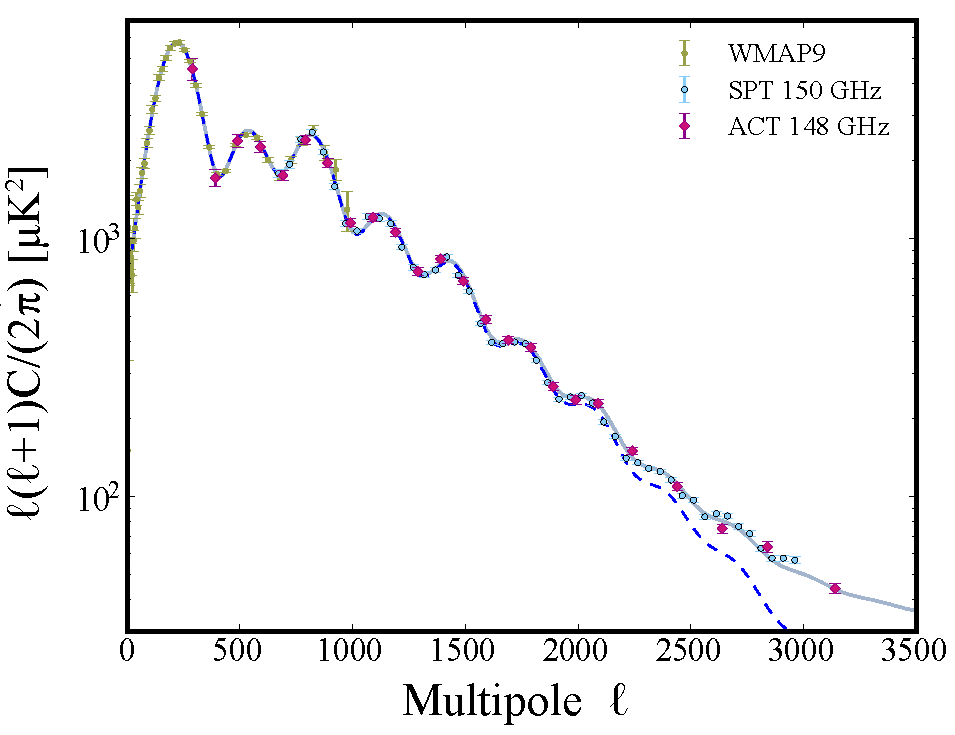
\includegraphics[width = .8\textwidth]{Figures/temp_power_spectrum.pdf}
    \caption{The CMB temperature power spectra measured by WMAP (yellow), the South Pole Telescope (blue) and the Atacama Cosmology Telescope (purple)~\cite{Das_2014}.  The temperature anisotropies of the CMB will be measured with the Simons Observatory and CMB-S4, two upcoming cosmology experiments, with further precision.}
    \label{fig:measured_cmb_spec}
\end{figure}

The shape of the CMB power spectra unlocks properties of the early universe.  For example, the first peak in the power spectrum at around $\ell\approx220$ corresponds to the angle at which we observe the sound horizon, or the distance that sound can travel between the big bang and recombination.  The measurement of this power spectrum's morphology can also determine physical matter and baryon densities.  The dark energy properties of our universe can be constrained by the power spectrum peak, as the dark energy and matter densities jointly alter the distance to last scattering~\cite{Hadzhiyska_2019}.  The matter denstiy of the universe alters the expansion of the universe, which determines when the universe reaches the temperature of last scattering, or when photons begin to stream freely.  The smaller angular scale distortions are in part due to an inhomogeneous universe at the time of last scattering ($z\approx 1100$).  

\section{The Polarized CMB}

The CMB is predicted to be polarized, due to Thompson scattering by free electrons during the era of recombination~\cite{weinberg_cosmo,Page_2007}.  Measuring this polarization would indicate the beginning of reionization and further have the potential to uncover primordial gravitational waves.  Just as the CMB's temperature spectrum is decomposed in spherical harmonics, we also decompose the polarized components.  We refer to the CMB's polarization signals as ``E-modes" and ``B-modes" after their likeness to curl-free (electric) and divergence-free (magnetic) fields (Figure~\ref{fig:e_b_pol}).
\begin{figure}
    \centering
    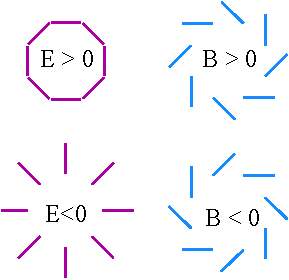
\includegraphics[width = .45\textwidth]{Figures/EB_pol.pdf}
    \caption{The polarization modes of the CMB.  The E modes have no curl, while the B modes have no divergence.  The polarization pattern in the CMB is caused by...}
    \label{fig:e_b_pol}
\end{figure}

The E-modes are produced by the density perturbations via Thompson scattering from a local quadrupole.  For this reason, the EE spectra peaks when scattering is highest, and when velocity is highest, between the two temperature spectrum peaks.  Primordial gravitational waves produce B-modes through Thompson scattering.  Further, the large-scale structure gravitationally lenses CMB photons traveling through, adding to the B-mode polarization spectra.  The scalar-to-tensor ratio, $r$, is directly determined through measurements of the B-mode polarization, as scalar perturbations generate E-mode polarization.

Let's now define the polarization signal basis of E- and B-modes.  The electric field of a photon travelling in the $\hat{z}$-direction is described by
\begin{equation}
    \Vec{E} = (E_x\hat{x} + E_y\hat{y})e^{i k_z - \omega t } \text{ .}
    \label{eq:e_photon}
\end{equation}
The Stokes parameters make up the basis of a photon's polarization, which is obtained from the electric field $\Vec{E}$, with parameters: intensity $I$, linear polarization $Q$, diagonal polarization $U$, and circular polarization $V$ (Eq.~\ref{eq:e_photon} and Eq.~\ref{eq:stokes}).

\begin{equation}
\begin{split}
    I & = |E_x|^2 + |E_y|^2 \\
    Q & = |E_x|^2 - |E_y|^2 \\
    U & = E_x E_y^* + E_x^*E_y\\
    V & = i(E_x E_y^* - E_x^*E_y) \\
\end{split}
\label{eq:stokes}
\end{equation}

The CMB should not carry any circular polarization, but can occur due to secondary mechanisms which take place after the surface of last scattering.  Just as the temperature power spectrum is decomposed into spherical harmonics, we express the polarization of the CMB in terms of spin-2 (where $a^*_{-2,\ell m} = a_{2,\ell m}$) spherical harmonics:
\begin{equation}
(Q \pm iU) = \sum_{\ell m}^{\pm 2} a^{\pm 2}_{\ell ,m} Y_{\pm2,\ell m} \text{ ,}
\end{equation}
where the expansion coefficients $a_{\ell m }^E$ and $a_{\ell m }^B$ are defined as
\begin{equation}
\begin{split}
    a_{\ell m }^E & = -\frac{1}{2}(a_{\ell m}^2 + a_{\ell m}^{-2}) \\
    a_{\ell m }^B & = \frac{i}{2}(a_{\ell m}^2 - a_{\ell m}^{-2}) \text{ .}
\end{split}
\end{equation}
The E- and B-modes of the CMB are then defined as
\begin{equation}
\begin{split}
    E(\theta,\phi) & = \sum_{\ell m} a_{\ell m }^E Y_{\ell m}(\theta,\phi) \\
    B(\theta,\phi) & = \sum_{\ell m} a_{\ell m }^B Y_{\ell m}(\theta,\phi) \text{ .}
\end{split}
\end{equation}
It follows that the CMB's polarized spectra are then defined as
\begin{equation}
    C_{\ell}^{XY} = \frac{1}{2\ell+1}\sum_m \langle a_{\ell m}^{X} a_{\ell m}^{Y*} \rangle 
\end{equation}
Here, $X$ and $Y$ can either be E-mode, B-mode, or temperature T spectra of the CMB, indicating cross-correlated spectra.

\section{Why Care About Beams?}
Every camera has a ``beam" (or optical response) which determines the optical performance (how your picture will turn out).  The smaller your beam, the higher the resolution of your picture.   The Field-of-View (FOV) determines how wide your picture can be.  The noise of your camera's detector determines how grainy the picture comes out.  All of these optical properties are defined by the camera's beam.  To take a picture of the CMB, the telescope is our camera; the beam of the instrument determines the optical performance at a given angular scale.  

This not only affects the immediate quality of our CMB maps, but also impacts the ability to study cosmological science.  Let's consider two cosmological parameters: the spectral index of inflation $n_{s}$, and the number of relativistic species $N_{\text{eff}}$.  The spectral index of inflation $n_{s}$ describes how fluctuations vary with angular scale.  Figure~\ref{fig:cmb_ns} shows the CMB power spectra at three different values of $n_{s}$ and at two different values of $N_{\text{eff}}$.
The red curve plots the achieved sensitivty of Planck for determining the spectral index $n_\text{s}$ and $N_{\text{eff}}$, showing $n_s\pm\sigma_{n_s}$, and $N_{\text{eff}}\pm\sigma_{N_{\text{eff}}}$.  The science goals of SO are plotted in blue to show the increase in sensitivity compared to Planck.  The right-most plot then shows that a mischaracterization of the instrument's beam can mimic the aforementioned uncertainties.  At small angular scales (large $\ell$ values), slight variations of $n_{s}$ change the slope of the power spectrum (Figure~\ref{fig:cmb_ns}).  For this reason, the beam must be well understood and characterized to achieve such ambitious science goals.

\begin{figure}[t!]
    \centering
    \includegraphics[width = \textwidth]{Figures/beam_neff.pdf}
    \caption{The simulated CMB power spectrum at varying spectral index of inflation $n_\text{s}$, and varying relativistic species $N_{\text{eff}}$.  Simulations are made with CAMB~\cite{camb_online} and show the $TT$ spectrum's deviation from nominal values, with $n_s\pm\sigma_{n_s}$, and $N_{\text{eff}}\pm\sigma_{N_{\text{eff}}}$.  In red is the sensitivity achieved by Planck, and in blue is the sensitivity goal of Simons Observatory.  The right-most panel simulates a mischaracterized instrument beam and how it can mimic deviations in the $TT$ spectrum of the CMB.}
    \label{fig:cmb_ns}
\end{figure}

Entire classes of inflationary models can be ruled out by constraining $n_{s}$.  Achieving this goal, however, requires precise beam calibration on these small angular scales.  Further, characterizing the polarization leakage from the telescope's beam is critical to map the tiniest signals of the CMB's polarization.  For this reason, this work focuses on beam calibration, both for the Simons Observatory and the Atacama Cosmology Telescope.

\section{Status of the Field}
\begin{table}[b!]
    \centering
    \begin{tabular}{|c|c|c|}\hline 
         Parameter & Planck 2018 Release & ACT 2020 Release \\ \hline
         $100\,\Omega_b h^2$ &  2.241$\pm$0.015 &2.153$\pm$0.030 \\
         $100\,\Omega_c h^2$ & 11.97$\pm$0.14 & 11.78$\pm$ 0.38\\
         $\ln(10^{10}A_s)$ &3.040$\pm$0.016& 3.050$\pm$0.030\\
         $\Omega_\Lambda$ & 0.687$\pm$0.008 & 0.696$\pm$0.022\\
         $n_{s}$ & 0.967$\pm$0.004 & 1.008$\pm$0.005\\
         $100\,\theta_{*}$ & 1.0410$\pm$0.00046 &1.0425$\pm$0.0007 \\
         $\tau$  &0.052$\pm$0.008 &0.065$\pm$0.014 \\
         $t_0$& 13.791$\pm$0.025 & 13.832$\pm$0.047\\
         \hline
    \end{tabular}
    \caption{The most recent cosmological parameters as from the 2018 Planck release~\cite{planck2020} and the 2020 ACT release~\cite{aiola_2020}.  Baryonic and cold dark matter densities $\Omega_b$, $\Omega_c$, dark energy density $\Omega_\Lambda$ spectral index of inflation $n_{s}$, acoustic horizon at decoupling $\theta_*$, reionization depth $\tau$, and the age of the Universe in Gyr, $t_0$.}
    \label{tab:cosmology_recent_results}
\end{table}

Since the detection by Penzias and Wilson in 1965, the cosmology community has made leaps to constrain the black-body of the CMB.  The Cosmic Background Explorer (COBE) was the first to measure the CMB power spectrum from space.  Since COBE, the measurement of fluctuations in the CMB has increased in precision, with experiments like WMAP, Planck, for example.  The South Pole Telescope and the Atacama Cosmology Telescope, two ground-based telescopes, have pushed the measurement further with increased resolution mapping of the sky.

In the coming years, cosmologists aim to detect the tiniest signals of the polarized CMB.  An ongoing challenge in cosmology instrumentation has been characterizing the polarization spectra of the CMB.  Specifically, the B-mode polarization of the CMB offers a unique window into early-universe physics~\cite{weinberg_cosmo}.  Because scalar perturbations generate E-mode polarization, a measurement of the B-mode polarization directly quantifies the scalar-to-tensor ratio, $r$.  The BB-power spectra has been reported by the Polarbear, South Pole Telescope and ACTPol collaborations~\cite{planck_data,choi_2020,PARAde_2014}.

\section{Outline of Thesis}

First, I overview two ground-based cosmology experiments in Chapter~\ref{ch:instruments}: the Atacama Cosmology Telescope (ACT) and the Simons Observatory (SO).  This work focuses on the development and characterization of optical components for the SO.  In the final chapter of this work, I characterize the optical performance of ACT.

In Chapter~\ref{ch:mma}, I present an overview of the meta-material absorbers used in the SO Large Aperture Telescope optics tubes to control stray light.  I also present the characterization of their optical properties using a radio holography receiver.  These tiles are comprised of an outer metamaterial layer, which approximates a lossy gradient index anti-reflection coating. They are fabricated via injection molding commercially-available carbon-loaded polyurethane (25\% by mass). The injection molding technology enables mass production at low cost.  Room temperature optical measurements verify their control of reflectance to less than 1\% up to 65$^{\circ}$ angles of incidence, and control of wide angle scattering below 0.01\%.

The characterization of optical components is continued in Chapter~\ref{ch:si}, where I characterize the reflectivity and loss tangent measured in the W-band (80-125\,GHz) and D-band (125-180\,GHz) in two samples of float zone silicon with intrinsic stoichiometry - one irradiated by neutrons, which increases the resistivity by introducing crystalline defects, and the other unperturbed.  I find the loss tangent $\tan\delta$ of $2.8\times10^{-4}$ and $1.5\times10^{-5}$ for neutron-irradiated silicon and intrinsic silicon, respectively, both with an index of refraction of 3.41.  The results demonstrate the applicability of silicon as a warm optical component in millimeter-wave receivers.  The depth of the reflection nulls provides a sensitive measurement of dielectric losses.

In Chapter~\ref{ch:ot_holo}, I present near-field radio holography measurements of the SO LATR optics.  These measurements demonstrate that radio holography of complex millimeter-wave optical systems comprising cryogenic lenses, filters, and feed horns can provide detailed characterization of wave propagation before deployment.  I used the measured amplitude and phase, at 4\,K, of the receiver near-field beam pattern to predict two key performance parameters: 1) the amount of scattered light that will spill past the telescope to 300\,K and 2) the beam pattern expected from the receiver when fielded on the telescope.  These cryogenic measurements informed the removal of a filter, which led to improved optical efficiency and reduced side-lobes at the exit of the receiver.  This is the first time such parameters have been confirmed in the lab prior to deployment of a new receiver.

Chapter~\ref{ch:sat_holo} presents additional near-field radio holography measurements, this time on the Small Aperture Telescope (SAT) optics tube.  Using the identical holography setup as described in Chapter~\ref{ch:ot_holo}, I present preliminary characterization of the SAT's optical performance; more specifically, I predict two key performance parameters: 1) the beam profile in the near-field and 2) the far-field beam pattern of the telescope expected from the receiver.

Chapter~\ref{ch:holosim} presents Holosim-ML: a Python code for beam simulation and analysis of radio holography data from complex optical systems.  This code uses machine learning to efficiently determine the position of hundreds of mirror adjusters on multiple mirrors with few micrometer accuracy.  I apply this approach to the example of the SO 6\,m telescope.  The ML framework makes the analysis of these measurements from many receiver positions straightforward to analyze.  I present an example of the SO dual reflector optical system and demonstrated that this approach can yield $<5\,\mu m$ alignment errors, the requirement for SO science goals.

In Chapter~\ref{ch:actbeams}, I analyze maps from the Atacama Cosmology Telescope Data Release 6.  From the maps, I select point sources and stack them in order to determine the temperature and temperature-to-polarization beams of the instrument.  This method is compared to the planet-derived beams of ACT.  We find the temperature-to-polarization leakage beams are consistent between the two methods, indicating that the planet-derived beams are sufficient for subsequent cosmology analysis.  We also find a spatial dependence of the point sources in the window functions, which we investigate and present several explanations for what might be causing this effect.

Lastly, in Chapter~\ref{ch:conclusion}, I summarize the results from this work and discuss their implications for the future of precision cosmology.
\chapter{Instrument Overview}
\label{ch:instruments}

We are in the age of precision cosmology, and measurements of the CMB spectra continue to improve in sensitivity.  Now, to measure the CMB polarization anisotropies, scientists are pushing forward the sensitivity of the instruments by increasing detector numbers, improving detector sensitivity, and controlling optical systematics, to name a few.  For example, the Atacama Cosmology Telescope (ACT), a ground-based cosmology experiment, used roughly 3000 bolometric detectors.  The Simons Observatory is scaling its detector count up to more than 50,000 bolometric detectors in order to improve mapping speed and sensitivity.  Looking ahead, the CMB-S4 collaboration, a next-generation cosmology project, plans to scale up even further: to roughly 500,000 detectors.  This, along with the many other improvements in instrumentation, aim to detect the faintest signals of the CMB polarization spectra.

In this chapter, I describe two ground-based cosmology experiments covered in this work: the Atacama Cosmology Telescope (ACT), an operational cosmology experiment~\cite{act_inst}, and the Simons Observatory (SO), this generation's cutting-edge cosmology experiment~\cite{so19}.  I describe the Simons Observatory Large Aperture Telescope instrument further in Chapters~\ref{ch:mma},~\ref{ch:ot_holo}, and ~\ref{ch:holosim}, and the Small Aperture Telescope in Chapter~\ref{ch:sat_holo}.

\section{Atacama Cosmology Telescope}

\begin{figure*}[t]
    \centering
    \includegraphics[width = \textwidth]{Figures/act_inst_close.jpeg}
    \caption{The Atacama Cosmology Telescope, surrounded by its outer ground screen. The inner co-moving screen further shields the instrument from any stray-light.  The primary mirror is behind the co-moving screen.}
    \label{fig:act_site}
\end{figure*}

The Atacama Cosmology Telescope (ACT) is a millimeter-wave telescope located on Cerro Toco in the Atacama Desert of Chile at an altitude of 5190\,m.  The full ACT is shown in Figure~\ref{fig:act_site} and the ACT site in Figure~\ref{fig:act_so_site}.  Since its first observations in 2007, the telescope has seen two major instrumentation upgrades: 1) ACTPol and 2) Advanced ACT.  In Chapter~\ref{ch:actbeams}, I present the characterization of the ACT mid-frequency beam and polarization leakage using point-source stacking.

The Advanced ACT, or ``AdvACT", is an upgrade to ACT's three detector arrays and their optics.  Filters and lenses were replaced to operate with the four new multichroic arrays.  This upgrade mapped the CMB in bands from 28\,GHz to 280\,GHz, and mapped approximately half of the sky.  Along with improved angular resolution (1.4' at 150\,GHz and 7.1' at 28\,GHz), the detectors improved polarization and temperature sensitivity due to twice the original number of detectors.
\begin{figure*}[t]
    \centering
    \includegraphics[width=\textwidth]{Figures/Site_Drone_Picture_July_2019.jpeg}
    \caption{The Simons Observatory (SO) and Atacama Cosmology (ACT) site in the Atacama Desert, Chile. The ACT telescope sits within a ground-shield which can be sen in the bottom center.  The outer ground screen protects the telescope from stray light.  The inner co-moving ground-screen further protects the telescope from stray light during observations.}
    \label{fig:act_so_site}
\end{figure*}

Figure~\ref{fig:act_inst} shows the ray-trace of ACT's off-axis Gregorian geometry with two reflectors which guide photons into the receiver cabin; the 6\,m primary is made of 71 adjustable aluminum panels and the 2\,m secondary is made of 11 adjustable aluminum panels~\cite{act_inst}.  The off-axis optical design minimizes scattered power and therefore drastically improves detector sensitivity~\cite{fowler_2007}.  Within the receiver cabin, three cryogenic optics tubes re-image the sky onto the detector arrays~\cite{thornton_2016}.  Light first enters through a 6.4\,mm-thick ultra-high molecular weight polyethylene window, followed by a series of Infra-red (IR) blocking filters at 300\,K, 40\,K, and 4\,K, which reflect out-of-band signal in order to reduce loading on the detectors.  The focal plane of the optics tube is cooled to 100\,mK.   Table~\ref{tab:act} summarizes the optical properties of the ACTPol instrument.

\begin{figure}[t]
    \centering
    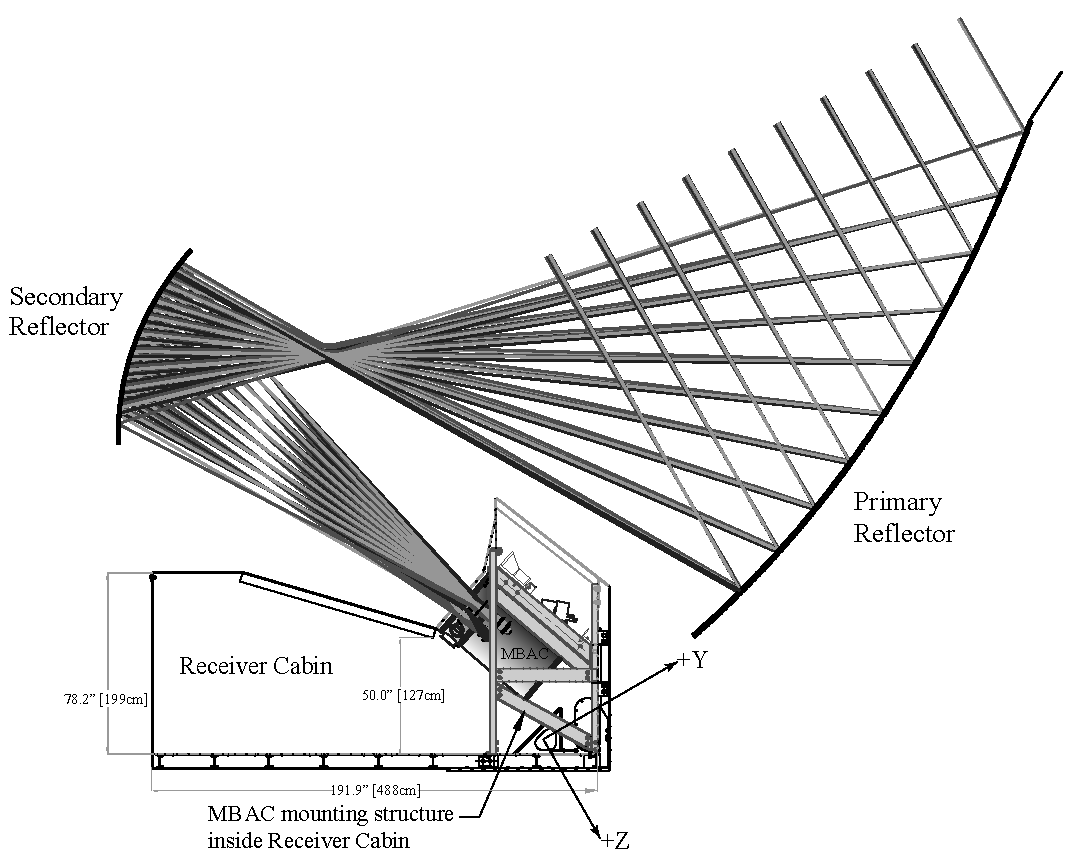
\includegraphics[width = \textwidth]{Figures/act_inst.pdf}
    \caption{Ray-trace diagram of the Atacama Cosmology Telescope~\cite{act_inst}.  The telescope is an off-axis Gregorian with two reflectors: the primary is 6\,m in diameter and the secondary 2\,m.  The rays trace into the Millimeter Bolometer Array Camera (MBAC) cryostat which houses the telescope's detectors.}
    \label{fig:act_inst}
\end{figure}

Since its inception in 2016, AdvACT has achieved many of its ambitious science goals~\cite{2016JLTP184772H}.  With improved sensitivity, ACTPol has measured the intrinsic temperature and polarization anisotropy at high-multipoles, which determines the spectral index of inflation, the primordial helium abundance, and neutrino properties~\cite{10.1117/12.857464}.  Galaxy clusters have also been studied from their Sunyaev-Zel’dovich effect, where CMB photons are scattered by high-energy electrons in the galaxy cluster along the line of sight~\cite{weinberg_cosmo}.  Soon to release its sixth data release (DR6), ACT has turned off observations and scientists will continue to use its groundbreaking data.

\begin{table}[b]
    \centering
    \begin{tabular}{|l|l|l|l|} \hline
        \textbf{ Parameter} & \textbf{MF}   &  \textbf{MF/HF}  & \textbf{HF}  \\ \hline \hline
        Number of Bolometers & 176 & 4430 &1006 \\\hline
        Angular Resolution (arcmin) & $7.1^{\prime}$/$4.8^{\prime}$ & $2.2^{\prime}$/$1.4^{\prime}$ & $0.9^{\prime}$ \\\hline
        Center Frequency (GHz) & 28/41 & 90/150 & 230\\\hline
    \end{tabular} \caption{ACT Key Characteristics~\cite{2016JLTP184772H}.}
    \label{tab:act}
\end{table}
\section{The Simons Observatory}
\begin{figure}[t]
    \centering
    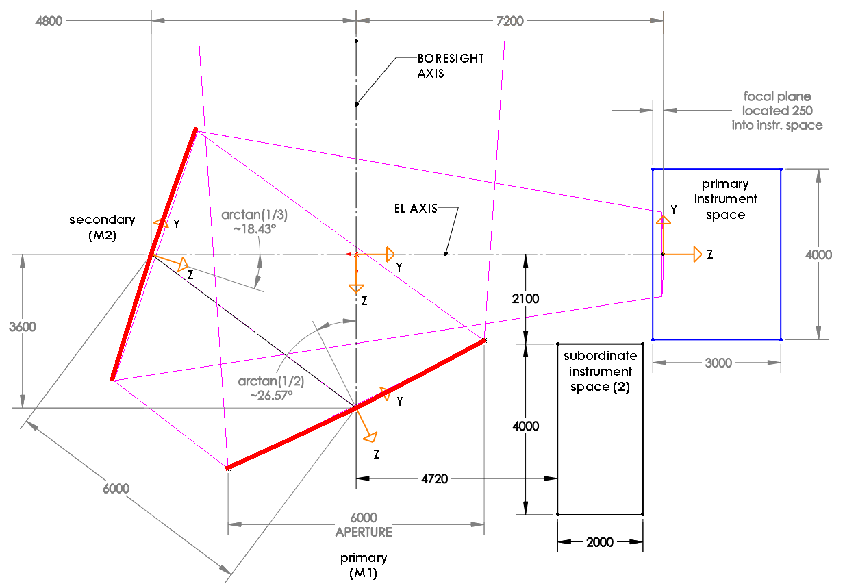
\includegraphics[width = .95\textwidth]{Figures/LAT_rt.pdf}
    \caption{Ray-trace diagram of the Simons Observatory Large Aperture Telescope~\cite{Parshley_2018}.  The telescope is a cross-Dragone with two reflectors, both 6\,m in diameter.  The rays trace into the Large Aperture Telescope Receiver (LATR) cryostat which houses 13 optics tubes.  The optics tubes guide the photons onto the detectors in the focal plane, which are cooled to 100\,mK.}
    \label{fig:so_inst}
\end{figure}
The Simons Observatory (SO) is a series of millimeter-wave telescopes designed to observe the Cosmic Microwave Background (CMB) temperature and polarization signals to an unprecedented sensitivity~\cite{gali18, so19}. With the combination of one Large Aperture Telescope (LAT)~\cite{xu/etal:2020c, zhu18, orlo18, coppi/etal:2018} and three Small Aperture Telescopes (SAT)~\cite{ali20}, the experiment will measure the temperature and polarization anisotropy of the cosmic microwave background with $\sim$\,70,000 background noise limited detectors operating at $\sim$\,100\,mK, covering six frequency bands centered on 27-280\,GHz (Table~\ref{tab:so}).

The resolution of SO will result in a catalog of extragalactic sources, including active galactic nuclei (AGN), dusty star-forming galaxies, and transient sources including Gamma Ray Burst (GRB) afterglows~\cite{so_science}.  SO expects to catalog 10,000-15,000 AGN sources at flux-densities above 7\,mJy~\cite{Tucci_2011}.  The low frequency coverage of SO will complement comparison work with other catalogs (e.g. VLA/VLASS, ASKAP/EMU, MeerKAT/MIGHTEE)~\cite{so_science}.  Dusty star-forming galaxies seen by SO will include local galaxies ($z<0.1)$ and high redshift galaxies (approximately $2<z<4$), and strong lensed galaxies beyond this range~\cite{Marrone_2017}.

\begin{table}[b]
    \centering
    \begin{tabular}{|l|l|l|l|} \hline
        \textbf{ Parameter} &  \textbf{LF} &  \textbf{MF}  &  \textbf{UHF}  \\ \hline \hline
        Number of Bolometers & $>$20,000& $>$20,000& $>$20,000\\\hline
        Angular Resolution (arcmin) & $3.3^{\prime}/3.0^{\prime}$ &$2.10^{\prime}/1.30^{\prime}$&$0.95^{\prime}/0.84^{\prime}$\\\hline
        Center Frequency (GHz) & 27/39 & 90/150 & 220/270\\\hline
    \end{tabular} \caption{SO Key Characteristics~\cite{Gudmundsson:21}.  The number of detectors are split evenly between the three frequency bands.  Note: the LF beam size is estimated by scaling down the MF and UHF beam sizes.}
    \label{tab:so}
\end{table}

\subsection{Large Aperture Telescope}

The Large Aperture Telescope (LAT) will map roughly 40\% of the sky at arcminute resolution~\cite{xu/etal:2020c}.   Figure~\ref{fig:so_inst} shows a cross-section and ray-trace of the LAT.  The primary mirror is 6\,m in diameter and constructed out of 77 individual adjustable panels, while the secondary mirror is 6\,m in diameter and constructed out of 69 adjustable panels \cite{gali18}.

Light from the sky is then reflected into the LAT Receiver (LATR), which houses up to thirteen optics tubes~\cite{Xu_2021}.  The LATR optics tubes re-image the optics onto the detector arrays (three detector arrays per optics tube).  Chapter~\ref{ch:ot_holo} presents radio holography measurements of the LAT optics tube, where I characterize the optical performance of the LAT Receiver optics tube.

\begin{figure*}[ht]
    \centering
    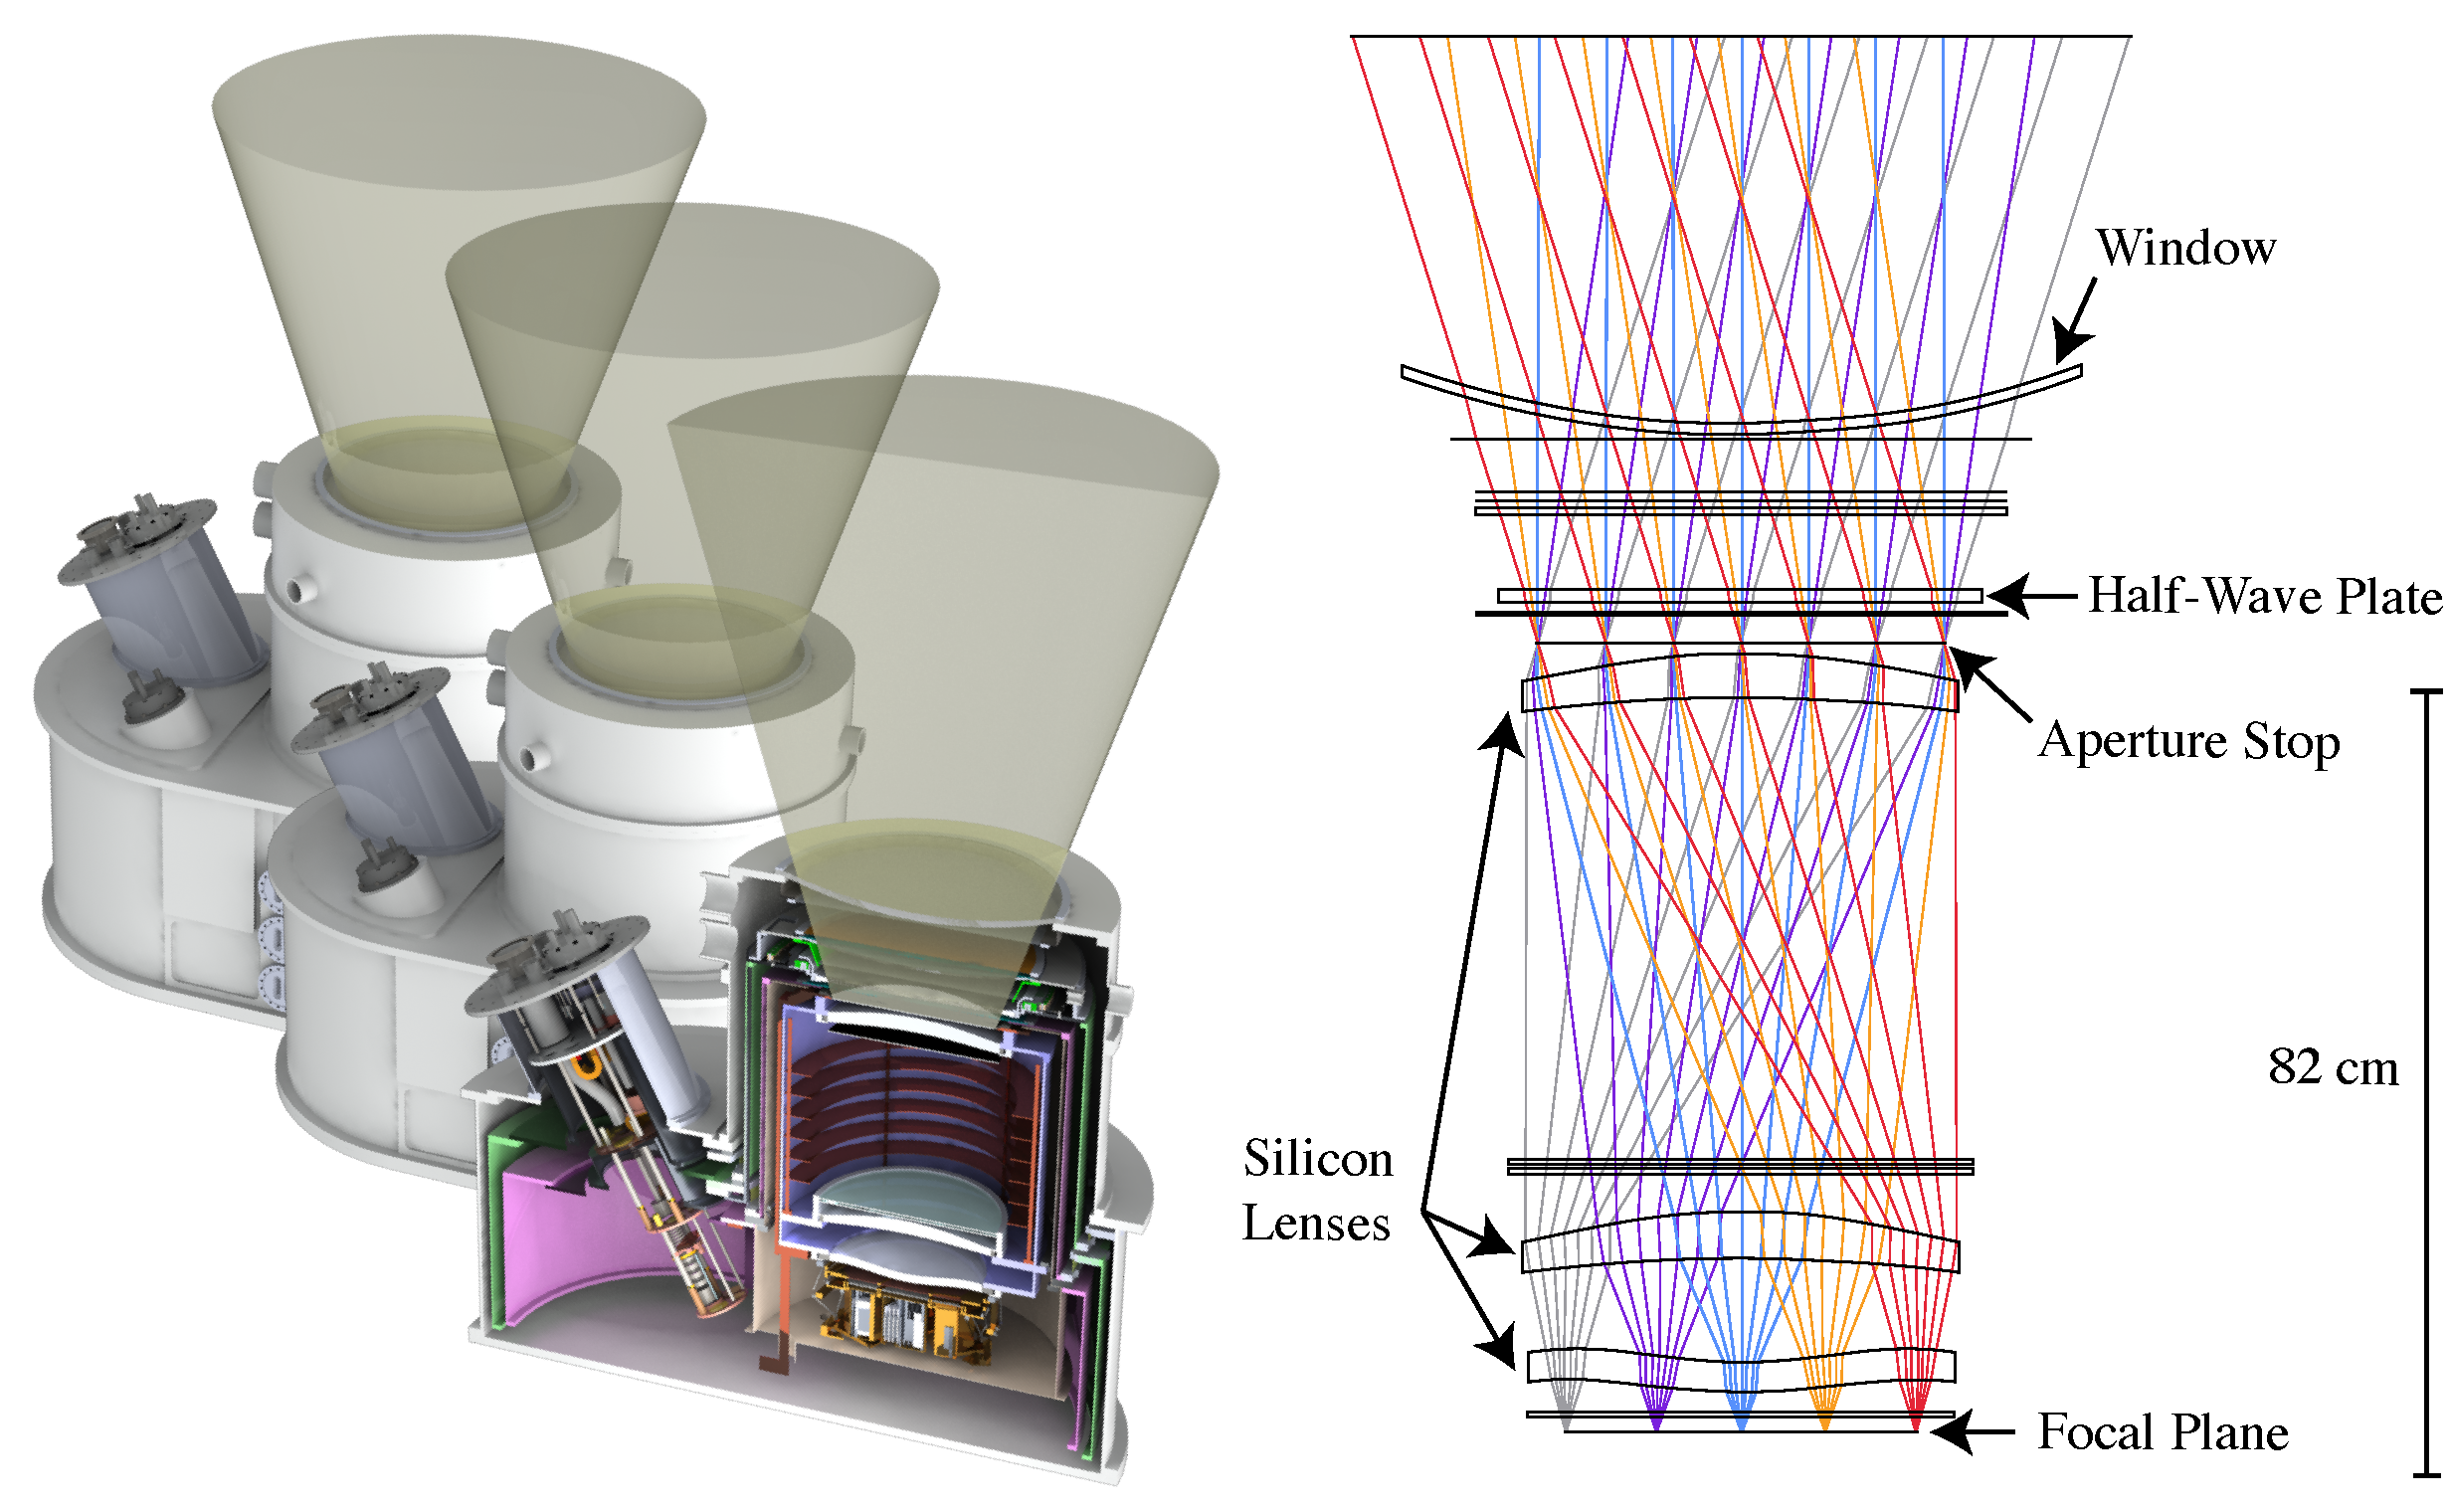
\includegraphics[width = \textwidth]{Figures/SAT3.pdf}
    \caption{Left: Three Small Aperture Telescope cryostats, with the front cross-section showing the inner optics tube.  Right: Ray-trace diagram of the Simons Observatory Small Aperture Telescope~\cite{2020SPIE11445E7LK}.}
    \label{fig:sat3s}
\end{figure*}

\subsection{Small Aperture Telescope}

The Small Aperture Telescope (SAT) optical design is a 0.42\,m diameter refractive telescope (Figure~\ref{fig:sat3s}).  Three SATs will measure the largest angular scales visible from the Atacama Desert.  In total, the three SAT's will hold roughly 30,000 cryogenic detectors, where the SAT is targeting to characterize the CMB on degree angular scales.  In Chapter~\ref{ch:sat_holo}, I present radio holography measurements of the SAT optics tube.

The SAT is a purely refractive telescope.  Figure~\ref{fig:sat3s} shows the ray-trace from the focal plane out the SAT window.  Light enters through a 3\,mm thick ultra-high molecular weight polyethylene hexagonal window with an anti-reflection coating~\cite{zhu18}.  A Cryogenic Half-Wave Plate (CHWP) polarization modulator then reconstructs the polarization of the CMB at 40\,K.  A 1\,K Lyot stop is the first cold optical element, and is followed by the SAT refractor.  Three anti-reflection coated silicon lenses~\cite{Datta:13,golec20} re-image the light onto seven hexagonal detector arrays.   Photons are then coupled onto the detectors by individual feedhorns.  The focal plane of each optics tube houses seven hexagonal detector arrays and are cooled to 100\,mK.

\subsection{The Status of the Simons Observatory}

The Simons Observatory is currently being deployed in the Parque Astronomico located in the Atacama Desert in Chile (Figure~\ref{fig:act_so_site}). The telescope site is situated at an elevation of 5,200 meters near the peak of Cerro Toco at $22 ^\circ$ 57' S, $67^\circ$47' W.  The arid conditions and elevation at the site minimize contamination to millimeter wave signals from water vapor.

Integration and testing occurs in parallel with deployment, as the rollout of the Simons Observatory continues.  In the year to come, SO will begin observations and characterize the CMB with unprecedented sensitivity, with many discoveries of the nature of our universe to come.
\chapter{Metamaterial Microwave Absorber (MMA) and its Cryogenic Applications}

\section{Introduction}
\section{Optical Design}
\section{Optical Testing}
\subsection{Optical Hardware}
\subsection{Receiver Electronics}
\subsection{Measurement}
\section{Reflection Measurement}
\section{Scattering Measurement}
\section{Future Applications}
\section{Conclusion}
\chapter{Reflectometry Measurements of the Loss Tangent in Silicon at Millimeter Wavelengths}
\section{Introduction}
\section{Procedure}
\subsection{Optical Hardware}
\subsection{Receiver Electronics}
\subsection{Samples: Neutron-irradiated and Intrinsic Silicon}
\section{Reflectometry and Transmissivity}
\subsection{Modeling}
\section{Results}

\chapter{The Simons Observatory: Characterization of Mid-Frequency Feedhorns}
\section{Introduction}
\section{Measurement Approach}
\subsection{Holography System}
\section{Results}
\subsection{Beam Maps}
\subsection{Cross-talk}
\section{Conclusion}
\chapter{The Simons Observatory: Characterizing the Large Aperture Telescope Receiver with Radio Holography}
\label{ch:ot_holo}
\section{Introduction}
\section{The SO Large Aperture Telescope Optics Tubes}
\section{Measurement Approach}
\subsection{Cryogenic Receiver}
\subsection{Holography System}
\section{Results and Interpretation}
\subsection{Propagation of Fields}
\subsubsection{Fields at Secondary Illumination}
\subsubsection{Far-Fields}
\section{Filter Removal}
\section{Public Code}
\subsection{Optics Simulation}
\subsection{Open Source Holography}
\section{Conclusion}
\chapter{The Simons Observatory Large Aperture Telescope}

\section{Introduction to Large Aperture Telescope}
\section{HoloSim-ML: machine learning applied to the efficient analysis of radio holography measurements of complex optical systems}
\subsection{Introduction}
\subsection{Motivation}
\subsection{Beam Simulation}
\subsection{Holography Analysis}
\subsection{Panel Fitting with Machine Learning}
\subsection{Measurement Practicalities and Robustness of Method}
\subsection{Public Code}
\subsection{Conclusion}
\chapter{Title of CMB Analysis Project}

\appendix

\include{Appendices/AppendixA}



\bibliographystyle{unsrt}
\bibliography{thebibliography.bib}


\end{document}